\documentclass[]{standalone}

% More defined colors
\usepackage[dvipsnames]{xcolor}
\definecolor{gray_black}{RGB}{18,54,147}
\definecolor{royal_blue}{RGB}{0,83,214}


\usepackage{tikz}
\usetikzlibrary{positioning, shapes.geometric, calc}

\tikzstyle{block} = [rectangle, rounded corners, minimum width=0.3cm, minimum height=0.3cm,
                    text centered, text width=2.3cm, line width=0.5mm, inner sep=0.15cm, draw=royal_blue, text=royal_blue]  %, text width=3cm
\tikzstyle{arrow} = [thick,-latex, gray_black]
\tikzstyle{tablecell} = [rectangle, line width=0.2mm, minimum width=0.5cm, minimum height=0.5cm, draw=black]

% \tikzstyle{Func} = [rectangle, rounded corners, minimum width = 6mm, minimum height = 6mm, draw=blue!50, fill = blue!20, inner sep = 0cm]
\tikzstyle{sum} = [circle, line width=0.3mm, minimum width = 6mm, minimum height = 6mm, draw=royal_blue, inner sep = 0cm, text = royal_blue]  % , fill = black!20

\begin{document}
 
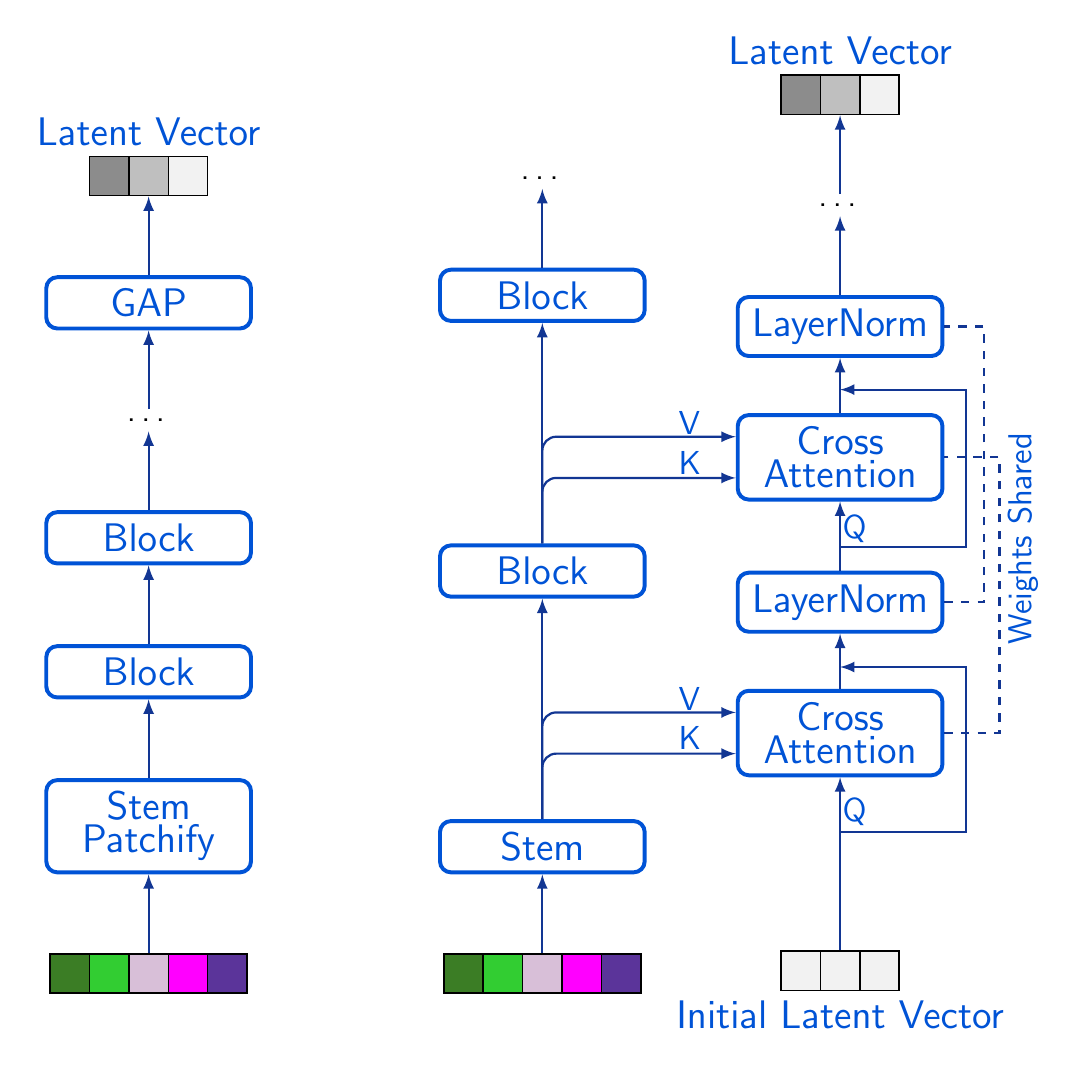
\begin{tikzpicture}
    
    % traditional isotropic neural networks
    \node[tablecell, fill = Thistle] (cell3) at (0,0){};  % input cell
    \node[tablecell, fill = LimeGreen] (cell2) [left = -0.2mm of cell3] {};   % input cell
    \node[tablecell, fill = OliveGreen] (cell1) [left = -0.2mm of cell2] {};   % input cell
    \node[tablecell, fill = Fuchsia] (cell4) [right = -0.2mm of cell3] {};   % input cell
    \node[tablecell, fill = RoyalPurple] (cell5) [right = -0.2mm of cell4] {};   % input cell
    % \node[text=royal_blue] (inputs) at (0,0) {\sffamily \Large Inputs};         % inputs node
    \node[block] (stem) [above = of cell3] {\sffamily \Large Stem \\ Patchify};            % stem node
    \node[block] (block1) [above = of stem] {\sffamily \Large Block};      % block1 node
    \node[block] (block2) [above = of block1] {\sffamily \Large Block};         % block2 node
    \node[] (dots) [above = of block2] {\sffamily \large \dots};                % dots node
    \node[block] (gap) [above = of dots] {\sffamily \Large GAP};                % gap node, Global Averaging Padding
    \node[tablecell, fill = gray!50] (end_cell2) [above = of gap] {};  % input cell
    \node[tablecell, fill = gray!90] (end_cell1) [left = -0.2mm of end_cell2] {};
    \node[tablecell, fill = gray!10] (end_cell3) [right = -0.2mm of end_cell2] {};
    \node[text=royal_blue] (output_latent) [above = 0 of end_cell2] {\sffamily \Large Latent Vector};

    \draw[arrow] (cell3) to (stem) ;
    \draw[arrow] (stem) to node[right, pos=0.2] {} (block1);  % \sffamily \large ($\dots,$N) 
    \draw[arrow] (block1) to node[right, pos=0.2] {} (block2);
    \draw[arrow] (block2) to (dots);
    \draw[arrow] (dots) to node[right, pos=0.7] {} (gap);
    \draw[arrow] (gap) to node[right, pos=0.3] {} (end_cell2);


    % isotropic neural networks with weight-shared iterative attentions
    \node[tablecell, fill = Thistle] (attn_cell3) at (5,0){};  % input cell
    \node[tablecell, fill = LimeGreen] (attn_cell2) [left = -0.2mm of attn_cell3] {};   % input cell
    \node[tablecell, fill = OliveGreen] (attn_cell1) [left = -0.2mm of attn_cell2] {};   % input cell
    \node[tablecell, fill = Fuchsia] (attn_cell4) [right = -0.2mm of attn_cell3] {};   % input cell
    \node[tablecell, fill = RoyalPurple] (attn_cell5) [right = -0.2mm of attn_cell4] {};   % input cell
    \node[block] (stem) [above = of attn_cell3] {\sffamily \Large Stem};            % stem node
    \node[block] (block1) [above = 2.8cm of stem] {\sffamily \Large Block};      % block1 node
    \node[block] (block2) [above = 2.8cm of block1] {\sffamily \Large Block};         % block2 node
    \node[] (dots) [above = of block2] {\sffamily \large \dots};                % dots node

    \draw[arrow] (attn_cell3) to (stem) ;
    \draw[arrow] (stem) to node[right, pos=0.2] {} (block1);
    \draw[arrow] (block1) to node[right, pos=0.2] {} (block2);
    \draw[arrow] (block2) to (dots);

    \node[block] (attn1) [above right = 1.6cm of stem, yshift=-6mm] {\sffamily \Large Cross \\ Attention};    % attention1 node
    \node[block] (layernorm1) [above = 0.7cm of attn1] {\sffamily \Large LayerNorm};                      % layernorm1 node

    \node[block] (attn2) [above right = 1.6cm of block1, yshift=-6mm] {\sffamily \Large Cross \\ Attention};  % attention2 node
    \node[block] (layernorm2) [above = 0.7cm of attn2] {\sffamily \Large LayerNorm};                      % layernorm2 node

    \node[] (dots2) [above = of layernorm2] {\sffamily \large \dots};                                   % dots node
    \node[tablecell, fill = gray!50] (attn_end_cell2) [above = of dots2] {};  % output cell
    \node[tablecell, fill = gray!90] (attn_end_cell1) [left = -0.2mm of attn_end_cell2] {};
    \node[tablecell, fill = gray!10] (attn_end_cell3) [right = -0.2mm of attn_end_cell2] {};
    \node[text=royal_blue] (output_latent) [above = 0 of attn_end_cell2] {\sffamily \Large Latent Vector};

    \node[tablecell, fill = gray!10] (attn_init_cell2) [below = 2.2cm of attn1] {};  % input cell
    \node[tablecell, fill = gray!10] (attn_init_cell1) [left = -0.2mm of attn_init_cell2] {};
    \node[tablecell, fill = gray!10] (attn_init_cell3) [right = -0.2mm of attn_init_cell2] {};
    \node[text=royal_blue] (init_latent) [below = 0 of attn_init_cell2] {\sffamily \Large Initial Latent Vector};     % init_latent node

    \draw[arrow, rounded corners=5pt] (stem) |- node[above right, pos=0.46, xshift=16mm, text=royal_blue, ] {\sffamily \large V} ([yshift=-3mm]attn1.north west);
    \draw[arrow, rounded corners=5pt] (stem) |- node[above right, pos=0.45, xshift=16mm, text=royal_blue, ] {\sffamily \large K} ([yshift=3mm]attn1.south west);
    \draw[arrow] (attn1) to (layernorm1);
    \draw[arrow] (layernorm1) to node[right, pos=0.6, xshift=-1mm, text=royal_blue,] {\sffamily \large Q } (attn2);

    \draw[arrow, rounded corners=5pt] (block1) |- node[above right, pos=0.46, xshift=16mm, text=royal_blue, ] {\sffamily \large V} ([yshift=-3mm]attn2.north west);
    \draw[arrow, rounded corners=5pt] (block1) |- node[above right, pos=0.45, xshift=16mm, text=royal_blue, ] {\sffamily \large K} ([yshift=3mm]attn2.south west);
    \draw[arrow] (attn2) to (layernorm2);

    \draw[arrow] (attn_init_cell2) to node[right, pos=0.8, xshift=-1mm, text=royal_blue,] {\sffamily \large Q } (attn1);
    \draw[arrow] (layernorm2) to (dots2);
    \draw[arrow] (dots2) to node[right, pos=0.3] {} (attn_end_cell2);

    \draw[arrow] ($(attn_init_cell2.north)+(0,1.5)$) -- ($(attn_init_cell2.north)+(1.6,1.5)$)  -- ($(attn_init_cell2.north)+(1.6,3.6)$)   -- ($(attn_init_cell2.north)+(0,3.6)$)  ;
    \draw[arrow] ($(layernorm1.north)+(0,0.3)$) -- ($(layernorm1.north)+(1.6,0.3)$)  -- ($(layernorm1.north)+(1.6,2.3)$)   -- ($(layernorm1.north)+(0,2.3)$)  ;
    \draw[thick, gray_black, dashed] ($(attn1.east)+(0,0)$) -- ($(attn1.east)+(0.7,0)$)  -- ($(attn2.east)+(0.7,0)$)   -- ($(attn2.east)+(0,0)$)  ;
    \draw[thick, gray_black, dashed] ($(layernorm1.east)+(0,0)$) -- ($(layernorm1.east)+(0.5,0)$)  -- ($(layernorm2.east)+(0.5,0)$)   -- ($(layernorm2.east)+(0,0)$)  ;
    \node[rotate=90, text=royal_blue] (weights_shared) [right = 1.0cm of attn1, xshift=10mm] {\sffamily \large Weights Shared};

\end{tikzpicture}

\end{document}